\subsubsection{Robotics}\label{ict:robotics:birk}
\index{Birk, Andreas}

\paragraph{Research Team}
Andreas Birk (Professor),
Kaustubh Pathak (Postdoctoral Fellow),
Winai Chonnaparamutt (PhD Student),
Mohammed Nour Abdel-Gwad Ahmed (PhD Student),
Max Pfingsthorn (PhD Student),
Jann Poppinga (PhD Student),
S\"{o}ren Schwertfeger (PhD Student) \\

The research of the Birk group focuses on Autonomous Systems. The work ranges from the
development of embedded hardware via mechatronics and sensors to high-level software. On
the basic research side of autonomous systems, machine learning and cooperation are core
activities. The robotics systems developed are used in various domains including
underwater and especially rescue robots.

 Especially mobile robots can be highly valuable tools in urban rescue
missions after catastrophes like earthquakes, bomb- or gas-explosions or daily incidents
like fires and road accidents involving hazardous materials. The robots are used to
inspect collapsed structures, to assess the situation and to search and locate
victims. There are many engineering and scientific challenges. Rescue robots not only have
to be designed for the harsh environmental conditions of disasters, but they also need
advanced capabilities like intelligent behaviors to free them from constant supervision by
operators.  IUB robotics is among the world-wide leading groups in this domain.

\paragraph{Highlights}

The IUB rescue robots demonstrated their capabilities on several
occasions including technology demonstrations, especially the Rescue
Robot Field Test Demo (figure~\ref{fig:outdoor}) and the European
Land Robotics Trials (ELROB). The robots also demonstrated their
capabilities at several competitions, namely three RoboCup events.
At the RoboCup US Open in Atlanta, the IUB team won the first place
in the rescue robot league, beating the favored US American groups.
The team also won the first place at the European RoboCup
competition, the Dutch Open in Eindhoven. The team also got the
Innovation Award at the RoboCup World Championship in Bremen for
demonstrating for the first time the successful combined usage of a
tele-operated with a fully autonomous robot at rescue missions. IUB
was the only European team that made it to the final round at the
RoboCup World Championship, and it was beaten in the end by Asian
teams that purely relied on tele-operated devices without any
on-board intelligence.



\begin{figure}[thpb]
  \centering
  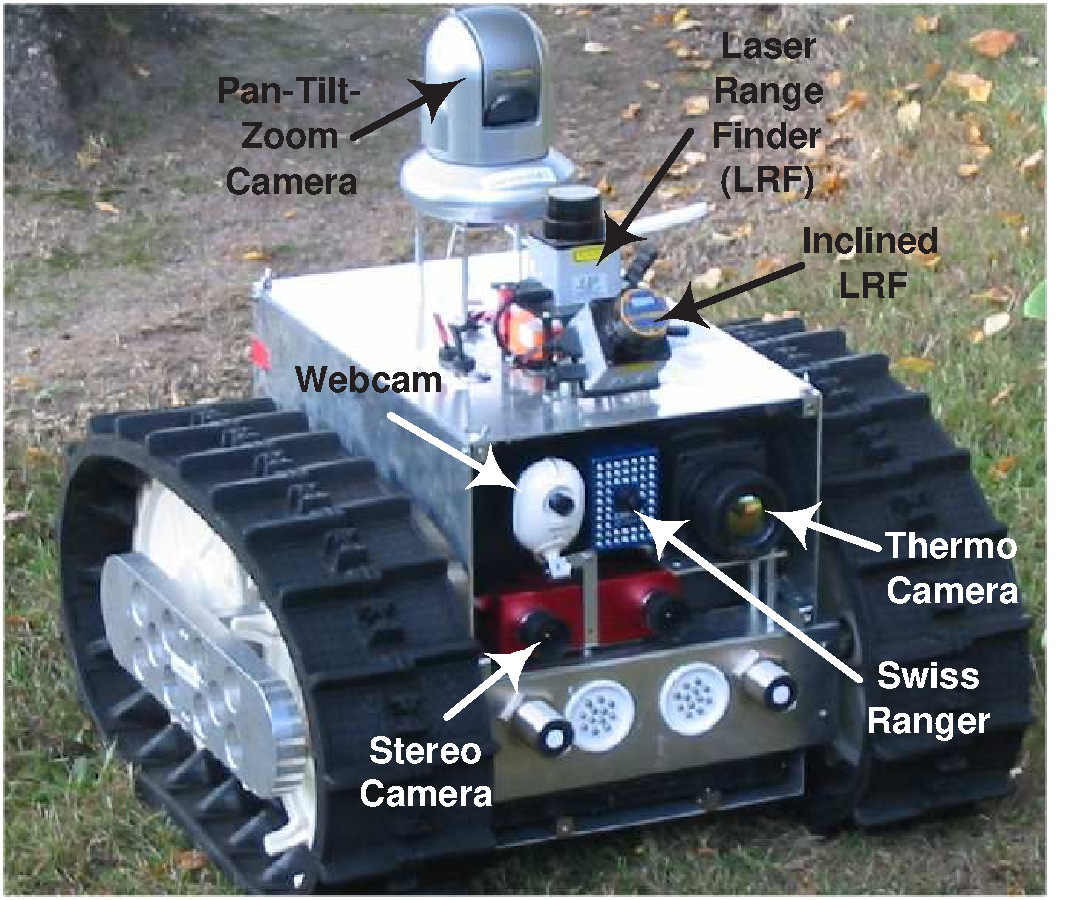
\includegraphics[width=\linewidth]{autonomousrobot.pdf}
  \caption{A {rugbot} with a selection of on-board sensors. Several sensors are dedicated
    to 3D range sensing to generate 3D environment models with a novel approach.}
  \label{fig:rugbot}
\end{figure}




On the research side, several contributions have been made ranging from the robot
mechatronics over on-board intelligence up to cooperative systems level.  Regarding the
mechatronics of the robots, a new locomotion system \cite{birk_flipper_rcup06} and a
special mobile communication system were developed \cite{birk_rescuecabledrum_rcup05}. The
latest type of robot from IUB robotics, the so-called rugbot, short for rugged robot, is
meanwhile one of the most advanced systems in this field \cite{birk_rugbot_ssrr06}. But
this holds not only for its mechatronic side but especially also with respect to its
on-board intelligence going up to full autonomy
\cite{birk_rescueteam_rcup05}. Contributions to several core topics for intelligent mobile
robot have been made in this context, especially for map generation
\cite{birkRescRobARJ06}, for the vectorization of maps
\cite{birk_mapvectorization_rcup06}, for the integration of autonomous behaviors with user
interactions \cite{birk_rescueGUI_rcup05}, and for the underlying architecture for
autonomy \cite{birk_autonomy_ssrr06}. The group also contributed to a high fidelity
simulator for mobile robots \cite{birk_virtualrobot_rcup05} that plays a significant role
in the prototype development of intelligent robot software.  Last but not least, work
regarding cooperative robot teams was done. The contributions include a novel algorithm
for multi robot exploration \cite{birk_CommExpore_CEP06} that can be used for search and
rescue missions by robot packs \cite{birk_commexplore_rcup05}. A second important result
is a novel algorithm for multi robot mapping \cite{BirkMultiMap_IEEEproc}.


\begin{figure*}
\centering
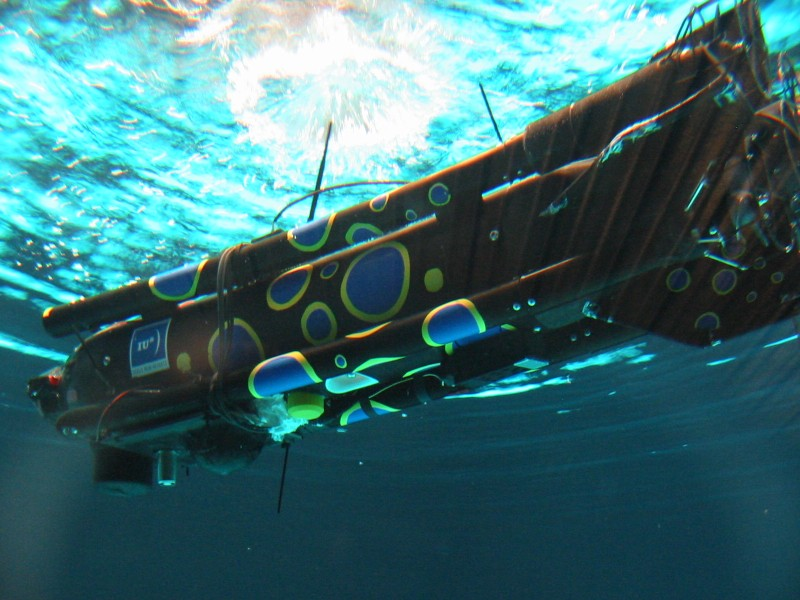
\includegraphics[width=.32\linewidth]{AUV-2006-best01.png}
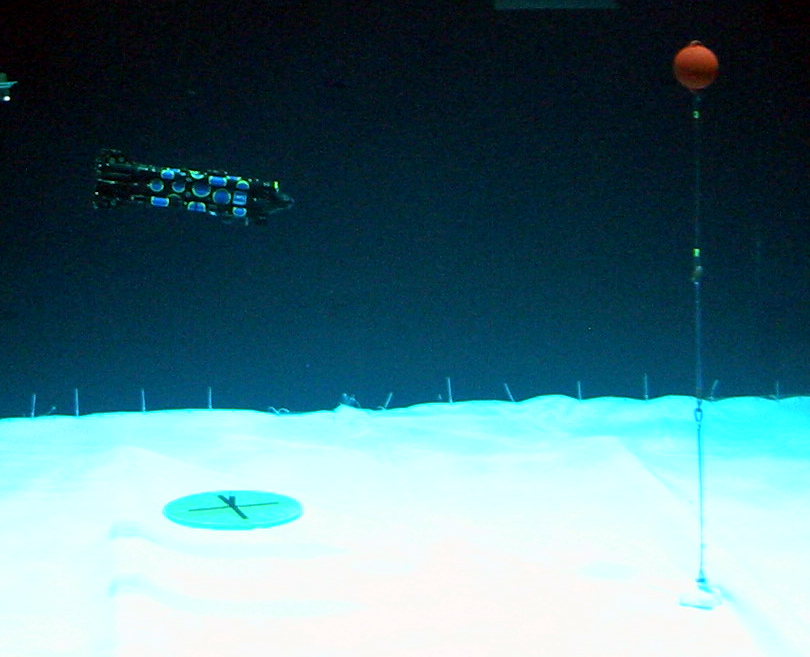
\includegraphics[width=.32\linewidth]{AUV-2006-best03.png}
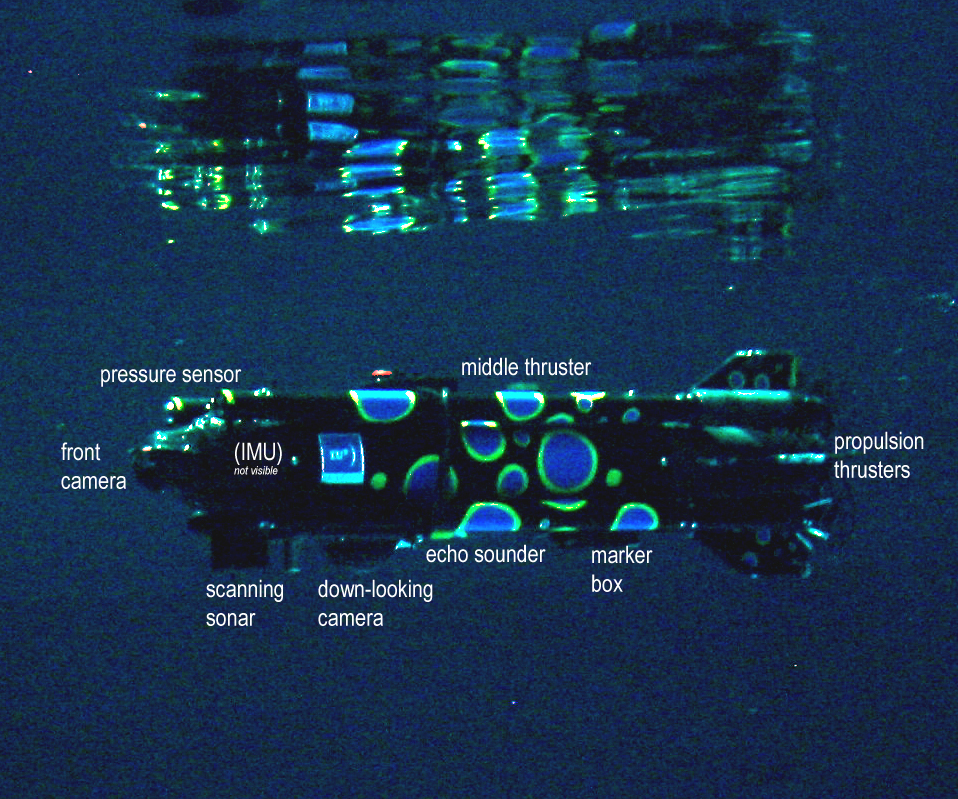
\includegraphics[width=.32\linewidth]{AUV-2006-best02-text.png}
\caption{The IUB-ATLAS Autonomous Underwater Vehicle (AUV) diving in a test pool
  (left). The AUV on an autonomous mission, searching for a midwater target in form of a
  submerged orange buoy (center). An overview of the main sensors of the AUV (right).}
\label{IUB-AUV}
\end{figure*}

IUB robotics made in 2006 also first successful practical steps in the domain of
underwater robotics by developing an Autonomous Underwater Vehicle (AUV). The work was
jointly done with ATLAS Elektronik in a cooperative project including also the IUB
robotics club. The most basic vehicle parts, namely the hull, the batteries, the motors
with propellers, and some sensors were provided to IUB by ATLAS. The on-board control
electronics and software were completely developed by IUB. This work is based on the
CubeSystem, a collection of hard- and software-components for fast robot prototyping,
which is also used for the IUB land robots. The AUV features fully autonomous motion
control and mission planning. It has an on-board vision system that allows to recognize
targets and to trigger appropriate behaviors. The system already successfully demonstrated
its capabilities at the Student Autonomous Underwater Challenge - Europe (SAUC-E), which
took place in August at the Pinewood movie studios near London.  The IUB-ATLAS-AUV came in
on second place in the performance evaluations, beating several of the established
underwater robotics research institutions.

\paragraph{Organization}
% list the (research) events you have organized, if any,

\begin{enumerate}
\item Chair ``RoboCup World Championship 2006, Rescue Robot League'', Bremen, Germany
\item Organizer ``Rescue Robot Field Test Demo'', opening event of RoboCup World
  Championship 2006, Bremen, Germany
\item Program Committee Member/Reviewer: Journal of Robotics and Autonomous Systems;
  Journal of Control Engineering Practice; International RoboCup Symposium; IEEE
  International Workshop on Safety, Security, and Rescue Robotics
\end{enumerate}

\paragraph{Collaborations}
\begin{enumerate}
\item {\sl International Rescue Systems Institute, Kobe, Japan}\\
  Prof. Satoshi Tadokoro\\
  Rescue Systems and Applications
\item {\sl University of Rome ``La Sapienza'', Italy}\\
  Prof. Daniele Nardi\\
  Autonomous Intelligent Functionalities within Rescue Robotics
\item {\sl Imperial College, London, UK}\\
  Dr. Yiannis Demiris, Senior Lecturer\\
  World Modeling by Autonomous Intelligent Systems
\end{enumerate}

\paragraph{Awards, Prizes}
\begin{enumerate}
\item Innovation Award, "Best Mixed Initiative Team"; RoboCup World Championship; Rescue
  Robot League; Bremen, Germany; July 2006
\item 1st Place Team; RoboCup US Open, Rescue Robot League; Atlanta, USA; April 2006
\item 1st Place Team; RoboCup Dutch Open, Rescue Robot League; Eindhoven, Netherlans; April 2006
\end{enumerate}

\paragraph{Grants}
% list the running grants in 2005, if none have been received, please delete this
% subsection.
\begin{enumerate}
\item Funded by DFG,  \emph{Learning of 3-Dimensional Maps of
Unstructured
Environments on a Mobile Robot}, May 2005 - April 2008 \\


\item Funded by DAAD-PPP,  \emph{3D Wordmodeling for Robot Action
Planning, Recognition and Imitation}, (July 2006 - June 2008) \\


\item Funded by private partner ATLAS Elektronik,
\emph{IUB-ATLAS Autonomous Underwater Vehicle}, (February 2006 - July 2006)\\


\item Funded by EU-IST NoE \emph{EUropean RObotics research
Network (EURON)}, (May 2004 - April 2008)

\end{enumerate}

%\paragraph{Publications}
% list the publications of 2005 (also accepted and in press), if none have been received, plese delete this
% subsection. Enter the publications into the SES publications database at
% http://kwarc.eecs.iu-bremen.de/ses-pubs/index.php and only reference them here.

%\begin{description}
%\item[Journals]
\nocite{BirkMultiMap_IEEEproc}
\nocite{birkRescRobARJ06}
\nocite{birk_CommExpore_CEP06}
%\item[Conference Proceedings]
\nocite{birk_rescueteam_rcup05}
\nocite{birk_rugbot_ssrr06}
\nocite{birk_autonomy_ssrr06}
%\item[Books/Collections]
\nocite{birk_commexplore_rcup05}
\nocite{birk_virtualrobot_rcup05}
\nocite{birk_rescueGUI_rcup05}
\nocite{birk_rescuecabledrum_rcup05}
\nocite{birk_flipper_rcup06}
\nocite{birk_mapvectorization_rcup06}
%\end{description}



























%\end{document}
%%% Local Variables:
%%% mode: latex
%%% TeX-master: "report"
%%% End:
